\documentclass[
    iai, % Saisir le nom de l'institut rattaché
    mi, % Saisir le nom de l'orientation
    %confidential, % Décommentez si le travail est confidentiel
]{heig-tb}

\usepackage[nooldvoltagedirection,european,americaninductors]{circuitikz}

\DeclareMathSymbol{*}{\mathbin}{symbols}{"01}   % Replace "*" with middle point


\signature{Paillard.svg} % Remplacer par votre propre signature vectorielle.

%\makenomenclature
\makenoidxglossaries
\makeindex

\addbibresource{bibliography.bib}

\newacronym{ao}{AO}{Adaptative Optics}

\newglossaryentry{heig-vd}{
    name=HEIG-VD,
    description={Haute École d'Ingénierie et de Gestion du canton de Vaud}
}
\newglossaryentry{hes-so}{
    name=HES-SO,
    description={Haute École Supérieure de Suisse Occidentale}
}
\newglossaryentry{IRSOL}{
    name=IRSOL,
    description={Istituto ricerche solari Aldo e Cele Daccò}
}

\newglossaryentry{PSF}{
    name=PSF,
    description={Point spread function}
}

% Auteur du document (étudiant-e) en projet de Bachelor
\author{Ervan Paillard}

% Activer l'option pour l'accord du féminin dans le texte
\genre{male}

% Titre de votre travail de Bachelor
\title{Optical turbulence analyzer for the IRSOL telescope}

% Le sous titre est optionnel
\subtitle{Bachelor thesis}

% Nom du professeur responsable
\teacher {Prof. L.Jolissaint de Sepibus (HEIG-VD)}

% Mettre à jour avec la date de rendu du travail
\date{\today}

% Numéro de TB
\thesis{11112}



\surroundwithmdframed{minted}

%% Début du document
\begin{document}
\selectlanguage{English}
\maketitle
\frontmatter
\clearemptydoublepage
%\newpage

%% Requis par les dispositions générales des travaux de Bachelor
\pagenumbering{Roman}


\preamble
\Authentication

%% Résumé / Résumé publiable / Version abrégée
\begin{abstract}
    % Francais
% Cette thèse, en complément à une thèse réalisée en parrallèle, a été réalisée dans le but de caractériser le site 
% d'observation astronomique de IRSOL (Tessin).
% L'objectif est de quantifier la perturbations atmosphérique du site d'observation.
% L'outil qui a été sélectionné est un système appelé DIMM (Differential image motion monitor). 
% Le principe est simple. Il suffit de masquer une image en deux pour en faire une mesure différentielle. 
% La mesure différentielle permet d'annuler les perturbations extérieures qui pourraient apparaîtres autour du télescope 
% (par exemple les mouvements et vibrations)
% La perturbation atmosphérique induira des mouvements de cette image et le seeing se qualifiera grace à l'écart type de la mesure.
% Le résultat pourra être exprimé avec l'écart type de l'angle d'incidence des faisceau ($\sigma$) ou par le paramètre de Fried ($r_0$) correspondant.
% Le projet a été mené a bien en réalisant un design optique et mécanqiue pour une adaptation sur le télescope de la HEIG-VD.
% Un programme a été constitué afin de traiter les données de l'image et de quantifier la perturbation. 
% Les résultats ...

% English
This thesis, in addition to a parallel thesis, was carried out to characterize the IRSOL astronomical observation site (Ticino).
The aim is to quantify the atmospheric disturbance at the observation site. \newline
The tool selected was a system called DIMM (Differential image motion monitor).
It principle is simple, an image is masked in two to produce a differential measurement.\newline
Differential measurement cancels out any external disturbances that may occur around the telescope (e.g. movements and vibrations).
\bigbreak
Atmospheric disturbance will induce movements in this image, and the seeing will be qualified by the standard deviation of the measurement.
The result can be expressed as the standard deviation of the beam incidence angle ($\sigma$) or as the corresponding Fried parameter ($r_0$).
\bigbreak
The project was completed with an optical and mechanical design for adaptation to the \Gls{heig-vd} telescope.
A program was created to process the image data and quantify the disturbance. \newline
The results ...
\end{abstract}

%% Sommaire et tables
\clearemptydoublepage
%\newpage

{
    \tableofcontents
    \let\cleardoublepage\clearpage
    \listoffigures
    \let\cleardoublepage\clearpage
    \listoftables
    \let\cleardoublepage\clearpage
    \listoflistings
}

\printnomenclature
\clearemptydoublepage
%\newpage

\printglossaries
\clearemptydoublepage
%\newpage

\pagenumbering{arabic}

%% Contenu
\mainmatter
\chapter{Introduction}
This chapter introduces the context and generalities relative to the work.

%====================================================================================================
% Context
%====================================================================================================
\section{Context}
This bachelor's thesis was carried out to support the research of the institute \Gls{IRSOL}. \newline
<<\Gls{IRSOL} is a research institute dependent on a foundation of the same name and affiliated to Università della Svizzera italiana.>>$^1$
The institute is based above Locarno in Ticino. \newline
Their research is mainly based on the measurement and characterization of the sun, and specializes in :
<<
\begin{enumerate}
    \item observational spectropolarimetry and instrument development,
    \item theoretical modeling of the generation and transfer of polarized radiation,
    \item numerical simulation of the solar atmosphere and numerical radiative transfer.
\end{enumerate}>>\footnote{|2| \Gls{IRSOL}, 2023. RESEARCH ACTIVITY, Research Activity at \Gls{IRSOL}. [Online]. [Accessed on 21.07.2023]. Available at: https://www.irsol.usi.ch/research/research-activity/}

The problem is that the institute is looking to expand its equipment in order to develop their research.
However, it is necessary to know the limitations of the measuring instruments, as well as the quality of the observation site.
Their first development objective would be to integrate an \acrfull{ao} system.
\newline
In odrer to asses the usefullness of \Gls{ao} two Bachelor thesis are conducted.
\begin{enumerate}
    \item "Caractérisation du télescope de l'observatoire solaire \Gls{IRSOL} (Tessin)" (Characterization of the \Gls{IRSOL} solar observatory telescope (Ticino))
    \item This thesis : "Analyseur de la turbulence optique pour le télescope solaire \Gls{IRSOL}" (Optical turbulence analyser for \Gls{IRSOL}'s solar telescope)
\end{enumerate}
The 1\textsuperscript{st} one is meant to measure the optical imperfections of the telescope itself and maybe of other optical equipment.
The 2\textsuperscript{nd} one aims to analyse optical turbulence on site.

Once these two projects are completed, \Gls{IRSOL} will be able to determine whether the acquisition of an \acrfull{ao} makes sense
and they will also be able to quantify the limiting element to their research (the observation site or the telescope).



%====================================================================================================
% Issue at hand
%====================================================================================================
\section{Issue at hand}
In a discussion with the institute, it was said: "Seeing evolves over the course of the day.
When the sun rises, the ground warms up and the heat rises. This is when seeing is at its worst.
But when the sun goes down, there's a moment when seeing is almost non-existent because the air currents freeze before going down again."
\bigbreak
The issue at hand is that the quality of the observation site is known but cannot be quantified.
The aim of this study is to quantify the quality of their observation site.
The instrument used will be the \Gls{DIMM} (Differential image motion monitor).

A \Gls{DIMM} works as follows (simplified version) :
\begin{enumerate}
    \item Capture an image masked by two small holes.
    \item Tracking the movement of these images.
    \item Measurement of the standard deviation of this movement.
    \item Conversion of previous result into turbulent layer thickness.
\end{enumerate}
The aim will be to play with the exposure time to determine the location of the image center, but also to freeze the turbulence.
\newline
Atmospheric turbulences will vary the centroid of the image, and it is this element that will be measured.
By taking the standard deviation of all these measurements, it is possible to give a result that qualifies the turbulence in a defined time.
\newline
The long explanation is the subject of this document.



\chapter{Theory}
%====================================================================================================
% Fundamentals
%====================================================================================================
\section{Fundamentals}
This parts goes over the fondamentals of optics necessary to understand futur developpments.
%====================================================================================================
% Seeing
%====================================================================================================
\subsection{Seeing}
\textbf{What's the seeing ?} : \newline In atmospheric optics, the "seeing" refers to the degree of blurring or distortion of astronomical objects
caused by Earth's atmosphere. The Earth's atmosphere is not homogeneous. It has various layers of air with different densities and temperatures.
Theses different layers causes the light passing throught it to be refracted in different ways. This result causes a constantly change of blurring,
distortion and glittering. Especially when looking an object low on the horizon. In our case, at IRSOL, the seeing is 4' of arc. We can go up
to 1' arc in the best case\newline
In general, seeing is determined by the angle of an object seen through the atmosphere, which is affected by factors such as temperature and wind speed.
The result of the seeing measure is the inverse of the "Fried parameter", wich describes the size of the atmospheric cells that cause the blurring.
When the Fried parameter is small, we could say that the seeing have good conditions. That means the image will have minimal blurring and distortion.
While poor seeing conditions have a larger Fried parameter, resulting in significant blurring and distortion of atmospherical objects.
%(Paramètre de Fried => Inverse)
\bigbreak
\textbf{Where are the turbulences} : \newline
First, we need to know how much type of turbulence we could see appearing and where they could be appear.\newline
There are 4 types of turbulence that we could see on the atmosphere. Each type is listed below :
\begin{itemize}
    \item Dome turbulence : \newline Appear when the air as not the same temperature between inside and outside the dome. This turbulence corresponds to
          the mirror turbulence.
    \item Surface trubulence : \newline Appear between the first 10 to 100 meters. Its appearance is due to the cooling by convection of the ground
          heated by the sun. Its minimum is just after the sunrise and its minimum when the sun sets. The evolution of this turbulence is an increasing
          evolution before the zenith and a decreasing evolution after it.\newline
          To counter this turbulence, a site selection is recommanded. For minimize it, the telescope could be place on a tower, away from any surface.
    \item Medium altitude turbulence : \newline Appear between 1.5 to 6 kilometers. Its appearance is due to atmospheric streams and in the thermal
          instabilities of the atmosphere. This turbulence is made up of multitudes of fine turbulent layers of varying densities and of a few hundred
          meters. For minimize it, a measure on the site should be carried out before.
    \item Tropopause and stratospheric turbulence : \newline Could appear between 6 and 20 kilometers. It reach a minimum t 6km and maximum on the
          tropopause between 10 and 20km. Its appearance is due to the strong winds shearing the atmosphere. This tubulence decrease after reach its maximum
          until it disappears after 25 - 30km.
\end{itemize}

%====================================================================================================
% DIMM
%====================================================================================================
\subsection{Differential image motion monitor (DIMM)}
\textbf{What's a DIMM ?} : \newline A differential image motion monitor is an instrument used in atmospheric optics to measure the amount of turbulence
in the Earth's atmosphere. It analyze the movement of stars as their light passes through the atmosphere, wich causes the stars to twinkle and blur.
\newline
The DIMM system consists of mask and split the image in two. After that, each image is recorded with a camera. On each part of this camera, the image
has a different seeing. Theses differences are used to determine the amount of distortion caused by the atmosphere.\newline
If we made a differential measure of theses images, we will get the atmospheric turbulence, wich is expressed as the seeing or the size of the
blurred image of a point source. \newline
The DIMM technique is widely used in astronomical observations, as it provides an objective and quantitative measure of the atmospheric turbulence,
which can affect the resolution and sensitivity of telescopes. It is also used in adaptive optics systems, where it is used to measure the atmospheric
turbulence in real-time, and to correct for the distortions using deformable mirrors.

\bigbreak
\textbf{Structures} : \newline the DIMM system is a relatively simple and robust instrument, which provides an accurate and objective measure of the atmospheric turbulence.
The elements that constitute a Differential Image Motion Monitor (DIMM) are listed below and viewable on the figure
\ref{fig:DIMM_Schematic} :
\begin{enumerate}
    \item Optical path : To create two images of our object, we need something wich will split our object in two. To realize this, a beam splitter could
          should be the best solution. It is also possible to separate the object before it enters the telescope by installing a "mask" before its first
          eyepiece.
    \item Camera : Which records the images of the star. The cameras are usually high-speed, sensitive detectors, such as CCDs or EMCCDs.
    \item Image processing software : The images obtained by the cameras are analyzed by software that measures the distortion caused by the atmosphere.
          The software calculates the difference in the distortion measurements obtained by the two telescopes, which allows for the determination of the
          atmospheric turbulence.
    \item Control and data acquisition system : The DIMM system is usually controlled by a computer, which also acquires and stores the data obtained by
          the cameras. The data can then be used to calculate the atmospheric turbulence, and to analyze the seeing conditions.
\end{enumerate}
\begin{figure}[H]
    \centering
    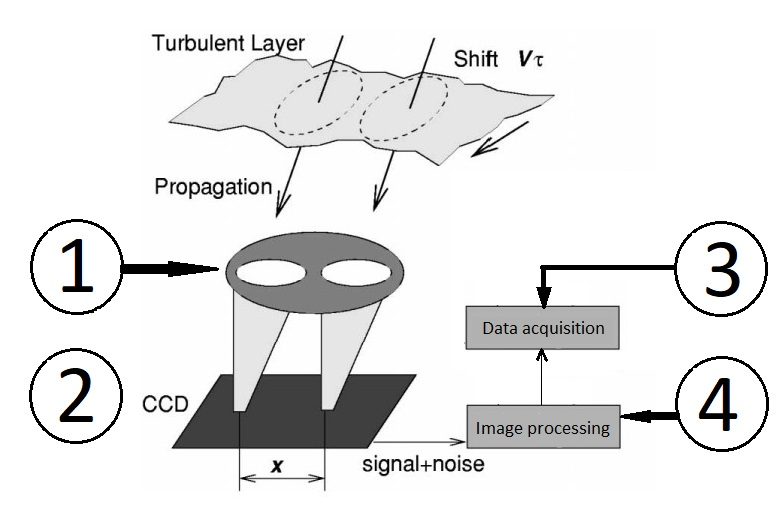
\includegraphics{assets/figures/Theory/DIMM_Schematic.jpg}
    \caption{Schematic principe of DIMM}
    \label{fig:DIMM_Schematic}
\end{figure}

\chapter{State of the art}
This chapter goes over a few solutions that already exist. Each aspect of the

\chapter{Conclusion}


\vfil
\hspace{8cm}\makeatletter\@author\makeatother\par
\hspace{8cm}\begin{minipage}{5cm}
    % Place pour signature numérique
    \printsignature
\end{minipage}

\clearpage
\printbibliography

\appendix
\appendixpage
\addappheadtotoc


\chapter{Première annexe}


\chapter{ assa}


\label{glossaire}
\printnoidxglossary
\label{index}
\printindex

% Le colophon est le dernier élément d'un document qui contient des notes de l'auteur concernant la mise en page et l'édition du document : il est parfaitement optionnel.
% \input{colophon.tex}

\end{document}
